\documentclass[dvisvgm,tikz,border=4pt]{standalone}
\usetikzlibrary{shadows,arrows.meta}
\begin{document}
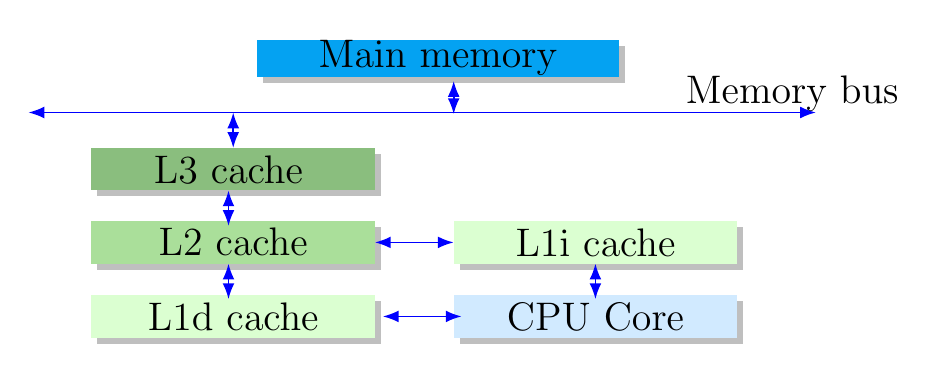
\begin{tikzpicture}[xscale=2]
  \fill[rotate=90, drop shadow, white!94!lime!87!green] (-0.6,0.3) rectangle (-0.06,-1.5);
  \fill[white!91!blue!90!cyan, rotate=90, drop shadow] (-1.54,0.3) rectangle (-1,-1.5);
  \node[node font=\Large] at (0.6,-1.27) {CPU\texttt{} Core};
  \fill[rotate=90, drop shadow, blue!82!darkgray!38!cyan] (1.77,1.55) rectangle (2.24,-0.75);
  \node[node font=\Large] at (-0.4,2.01) {Main memory};
  \node[node font=\Large] at (0.6,-0.33) {L1i cache};
  \node[node font=\Large] at (1.85,1.56) {Memory bus};
  \fill[rotate=90, drop shadow, white!94!lime!87!green] (-1.54,2.6) rectangle (-1,0.8);
  \node[node font=\Large] at (-1.7,-1.27) {L1d cache};
  \fill[rotate=90, drop shadow, white!82!purple!70!green] (-0.6,2.6) rectangle (-0.06,0.8);
  \node[node font=\Large] at (-1.7,-0.32) {L2 cache};
  \fill[rotate=90, drop shadow, orange!94!white!54!cyan] (0.33,2.6) rectangle (0.87,0.8);
  \node[node font=\Large] at (-1.73,0.6) {L3 cache};
  \draw[blue, arrows=Latex-Latex, semithick] (-3,1.32) -- (2,1.32);
  \draw[blue, arrows=Latex-Latex, semithick] (-0.3,1.72) -- (-0.3,1.3);
  \draw[blue, arrows=Latex-Latex, semithick] (-1.7,1.32) -- (-1.7,0.87);
  \draw[blue, arrows=Latex-Latex, semithick] (-1.73,0.33) -- (-1.73,-0.12);
  \draw[blue, arrows=Latex-Latex, semithick] (-0.25,-1.27) -- (-0.75,-1.27);
  \draw[blue, arrows=Latex-Latex, semithick] (-0.3,-0.33) -- (-0.8,-0.33);
  \draw[blue, arrows=Latex-Latex, semithick] (-1.73,-0.6) -- (-1.73,-1.05);
\draw[blue, arrows=Latex-Latex, semithick] (0.6,-0.6) -- (0.6,-1.05);
\end{tikzpicture}
\end{document}
